\chapter{Results}
\label{chap:results}
\section{Identification of \emph{M. edulis} hemocyte subpopulations according to side scatter (SSC) and forward scatter (FSC)}
\subsection{Eosinophilic granulocytes}


SD og absolute error


\begin{figure}[!ht]
    \centering
    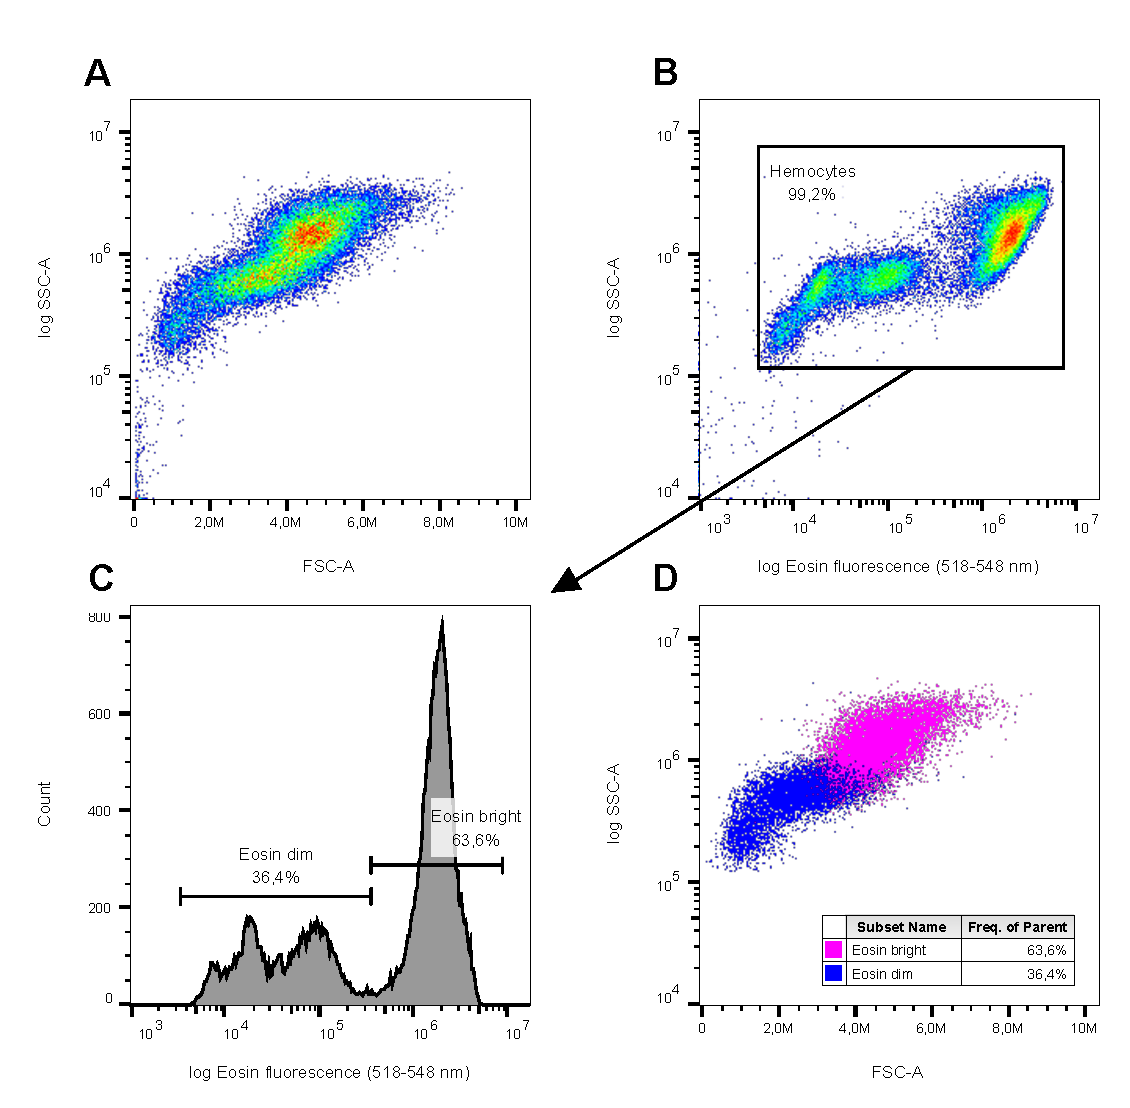
\includegraphics[width=1.0\textwidth]{figures/Eosin and Percoll exp/Eosin exp pool ex for Incskape test.pdf}
    \caption{\textbf{Identification eosinophilic granulocytes by flow cytometry based on eosin fluorescence. A} Representative light scatter profiles of... \textbf{B} }
    \label{fig:eosin_exp}
\end{figure}




\begin{figure}[!ht]
    \centering
    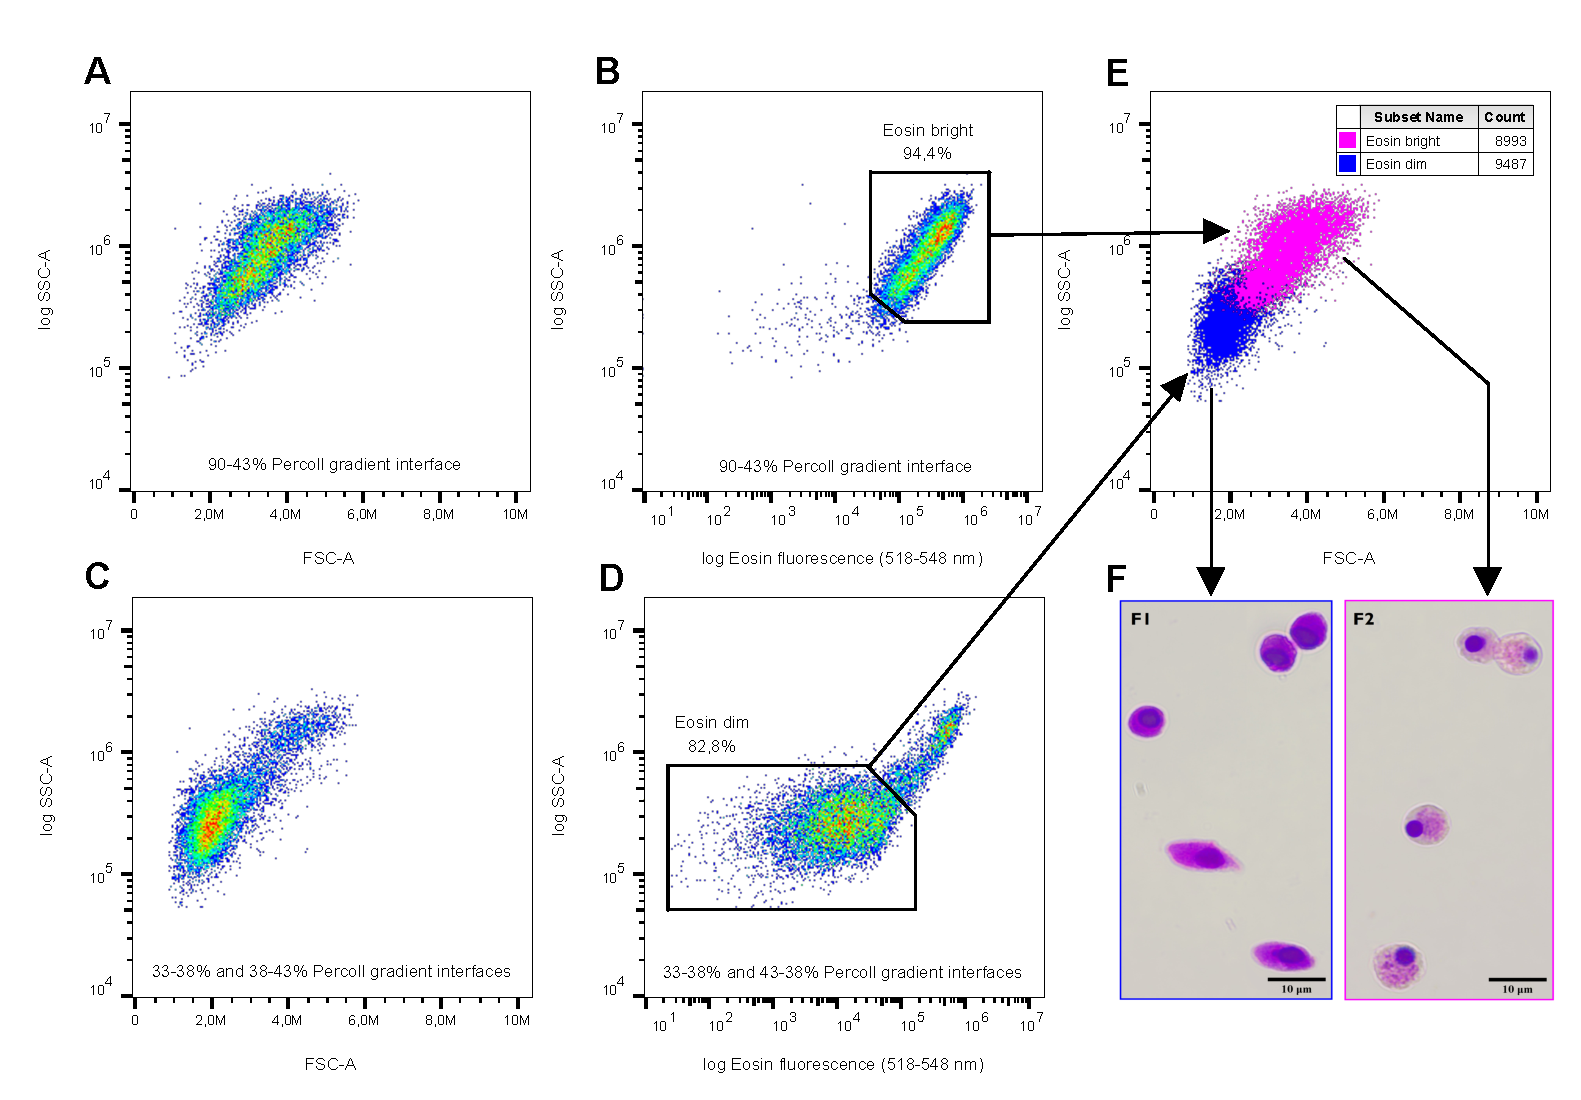
\includegraphics[width=1.0\textwidth]{figures/Eosin and Percoll exp/Percoll sep for Inkscape 2.pdf}
    \caption{\textbf{Confirmation of the light scattering profiles of eosinophilic and basophilic granulocytes pre-separated by discontinuous density centrifugation. A} Light scattering profile of the 95\% pure eosinophilic fraction that separated out on top of the 43-90\% Percoll gradient interface. \textbf{B} Bla bla bla eosin separation bla bla...}
    \label{fig:Percoll-dotplots}
\end{figure}







